% LED layout of one strip (example: left leg, autonomous flight, no error)
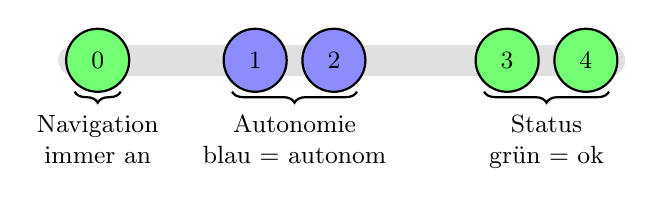
\begin{tikzpicture}[
    font=\small,
    led/.style={circle, draw, thick, minimum size=8mm, inner sep=0pt},
    brace/.style={decorate, decoration={brace, amplitude=4pt, mirror, raise=3pt}, thick},
]
    % wider gaps between the channel groups, so the labels below do not collide
    \draw[line width=4mm, black!12, line cap=round] (-0.3,0) -- (6.5,0); % the strip itself
    \node[led, fill=green!55] (l0) at (0.0,0) {0};
    \node[led, fill=blue!45]  (l1) at (2.0,0) {1};
    \node[led, fill=blue!45]  (l2) at (3.0,0) {2};
    \node[led, fill=green!55] (l3) at (5.2,0) {3};
    \node[led, fill=green!55] (l4) at (6.2,0) {4};

    \draw[brace] (l0.south west) -- (l0.south east)
        node[midway, below=8pt, align=center] {Navigation\\immer an};
    \draw[brace] (l1.south west) -- (l2.south east)
        node[midway, below=8pt, align=center] {Autonomie\\blau = autonom};
    \draw[brace] (l3.south west) -- (l4.south east)
        node[midway, below=8pt, align=center] {Status\\grün = ok};
\end{tikzpicture}
